%====================================================================================================
% ?????
%====================================================================================================
% TCC
%----------------------------------------------------------------------------------------------------
% Autor				: Jasane Schio
% Orientador		: Gedson Faria
% Co-Orientador		: Angelo Darcy
% Instituição 		: UFMS - Universidade Federal do Mato Grosso do Sul
% Departamento		: CPCX - Sistema de Informação
%----------------------------------------------------------------------------------------------------
% Data de criação	: 01 de Outubro de 2015
%====================================================================================================
% NO FUTURO
\chapter{Introdução} \label{Cap:Introducao}
Avanços tecnológicos tentam a cada dia mais dar vida as máquinas aplicando sentidos e percepções que se assemelham as humanas. Dentre estes, Inteligência Artificial, Aprendizado de Máquina, processamento de áudio, processamento de imagem entre outros. Segundo Albuquerque\cite{Albuquerque:2001} processar uma imagem, da mesma maneira que o nosso sistema visual humano é capaz de fazer é extremamente complexo, realizar as mesmas tarefas com a ajuda de máquinas, exige por antecedência uma compreensão “filosófica” do mundo ou dos conhecimentos humanos. Sem esse conhecimento pré existente por parte da máquina, a interpretação de uma imagem e seu processamento se baseia nas informações contidas na mesma.
	
	 Essa obtenção e entendimento das informações contidas na imagem se dá pela Visão Computacional, o ramo encarregado por simular o sistema visual humano. O que é feito de uma maneira única pelo sentido humano é separado em varias tarefas dentro da Visão Computacional com a captura de imagem, seu processamento, aquisição de informações da mesma, processamento dessa informação e aplicação de parâmetros para classificação da informação entre outros. Gonzalez\cite{Gonzalez:2008} descreve que uma imagem digital é composta por um número finito de elementos, cada um dos quais tem um determinado local e valor, assim o Processamento de Imagem Digital tem como tarefa a retirada de informações dos elementos de uma imagem.
	
	Dentre tipos de processamento de imagens existem, Gonzalez\cite{Gonzalez:2008} os define como: aplicações de ações primitivas de modificação de imagem, esta caraterizada por seu resultado final ser também uma imagem semelhante a imagem inicial porém modificada (Low-Level-Process), divisão de imagem em regiões e alguns tipos de reconhecimento e classificação de objetos, caraterizada por seu resultado final ser muitas vezes apenas regiões ou informações da imagem inicial (Mid-Level-Process), e o mais “sensorial” de todos que é a analise de objetos usando funções cognitivas associadas a visão computacional, essa usa informações relevantes para o reconhecimento de objetos (Higher-Level-Process).     
%
%	Neste trabalho propõe-se a realização de um processo de reconhecimento do objetos em imagens em tempo real coloridas com tempo de maquina reduzido. Este processamento irá ser realizado em imagens de futebol de robô da categoria Very Small Size, que serão processadas usando modelo de cores HPG e usando intervalos de valores de histograma de cores como parâmetro para detecção do objeto. O reconhecimento desses objetos também apresentara uma forma dinâmica de alocamento de equipes onde o sistema detectara os times e seus participantes de forma autônoma. 
 
	Neste trabalho propõe-se o a automatização do processo de detecção de objetos desenvolvendo um sistema de calibração de intervalo de Mínimos e Máximos dos valores HSV de cores para ser usado pela equipe de Futebol de Robôs Cedro, categoria Very Small Size. Valores HSV são um dos tipos de valores usados para definir as cores em computação, esses valores são correspondentemente Hue, a cor pura, Saturation, o grau de pureza da cor, e Lightness, que é o luminosidade aplicada. No sistema além da detecção automática estará também disponível a detecção manual de objetos. 


\section{Justificativa}
\begin{itemize}

%	\item A ausência de métodos que facilitem a calibração de corem nas bibliotecas de processamento de imagem já existentes
	\item A falta, na equipe, de um sistema de fácil manuseio para detecção de valores HSV
	\item A falta, na equipe, de um sistema automático de registro do valores HSV mínimos e máximos
	\item A falta, na equipe, de um sistema que defina mínimos e máximos de forma automática, baseando-se nos objetos escolhidos
	\item A falta, na equipe, de um sistema autônomo de calibração de intervalo de cores
	\item Aplicação do sistema proposto na identificação de robôs moveis em times de futebol de robôs.
	
			

\end{itemize}
\section{Objetivos} \label{Sec:Objetivos}

\subsection{Objetivo Geral} \label{Sec:ObjetivoGeral}
Este trabalho tem por objetivo principal automatizar o sistema de identificação de objetos 
coloridos em imagens provenientes de uma câmera  em tempo real, fazendo a calibração de intervalo de Mínimos e Máximos dos valores HSV.  
Para alcançar o objetivo principal, foram propostos os seguintes objetivos específicos.

\subsection{Objetivos Específicos} \label{Sec:ObjetivosEspecificos}

\begin{itemize}
	
%	\item Detecção e calculo dos valores mínimos e máximos para cada cor
	\item Implementar uma interface que conte com disposição de informações no estilo gráfico ou histograma de cores para um corte manual de valores
	visando diminuição da velocidade de detecção; 
	\item Estudo e implementação de um sistema inteligente de calibração de cores e no corte inteligente de valores minimo e máximo das cores
	\item Testar o sistema proposto para identificação de equipes e participantes do futebol 
	de robô na categoria Very Small Size. 
	
	
\end{itemize}

\newpage

\section{Trabalhos Corelatos}
Para o tema especifico deste trabalho, calibração de intervalo de cores para times de futebol de robos da categoria very small size, não foram encontrados trabalhos relacionados, porém foram encotrados Team Discription Papers e descrições de sistemas usados pelos times, onde consta sobre o processo de calibração e os metodos usados.

\subsection{Calibra}
O Centro Universitário da FEI, como visto em\cite{PenharbelTime}, utiliza em sua equipe Y04 utiliza um sistema, desenvolvido denominado CALIBRA\cite{Penharbel:2004}.Desenvolvido para sistemas Linux e com Graphical User Interface\cite{Penharbel:2004}, o sistema de calibração possui um modulo chamado de MainWindow, que é responsavel pela configuracao de brilho, cor e contraste da imagem adquirida pela camera e gera um arquivo que é analizado na hora da criacao das cores padrao\cite{PenharbelTime}, onde cores-padrão são definidas como intervalos no espaço de cores HSI\cite{PenharbelTime}.
\begin{figure}[!h]
	\centering
	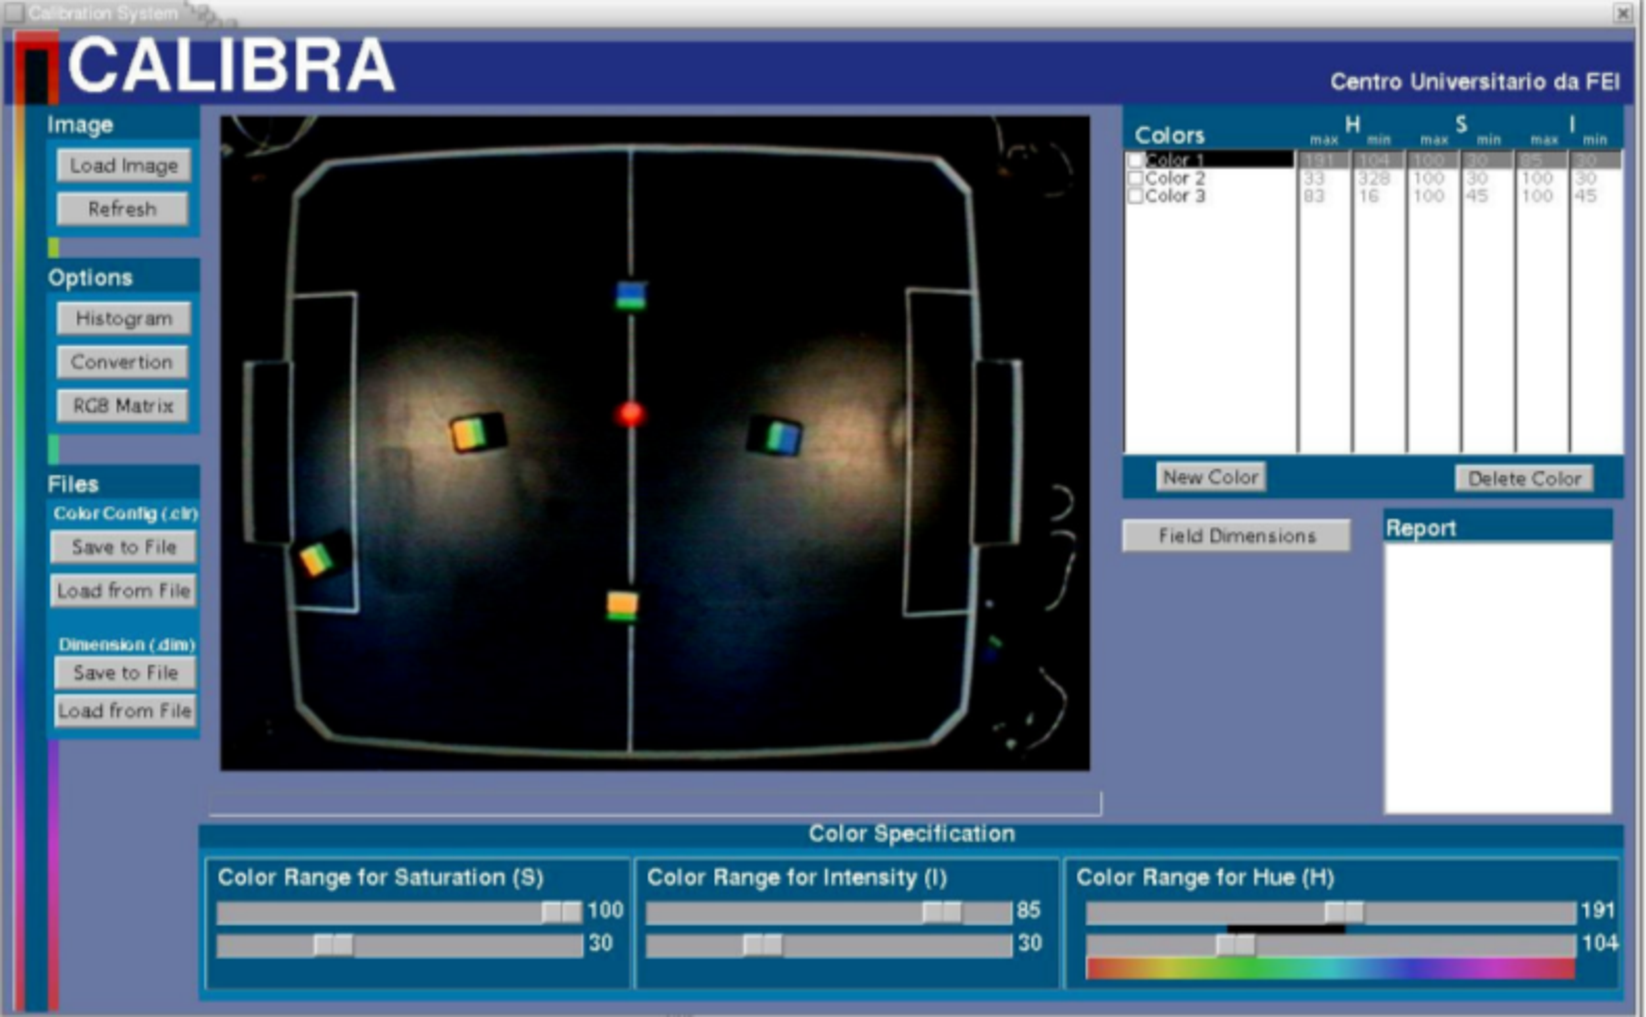
\includegraphics[width=0.6\textwidth]{calibra.pdf}
	\caption{Sistema Calibra desenvolvido pelo Centro Universitário da FEI \cite{Penharbel:2004}}
	\label{Calibra}
\end{figure}

\subsection{VSS-Vision}

Em 2015 Rosa\cite{Rosa:2015} descreve em seu Trabalho de Conclusão sobre a equipe de futebol de rob\^os Very Small Size, do Laboratório de Sistemas Inteligentes e Robótica, SIRLab(Faeterj-Petrópolis), o sistema de visão computacional da equipe, durante a competição do ano de 2014, que abrange inclusive a parte de calibração. 

\begin{figure}[!h]
	\centering
	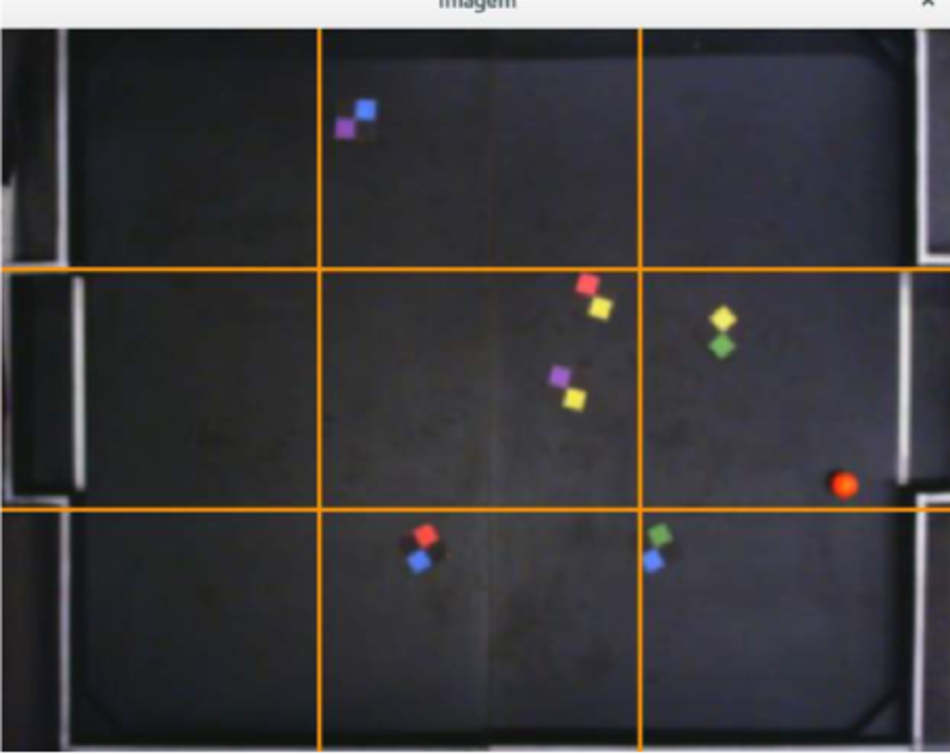
\includegraphics[width=0.4\textwidth]{vssvision.pdf} 	
	\caption{Sistema de calibracao desenvolvido peloSIRLab \cite{Rosa:2015}}
	\label{SIRLabCalibracao}
\end{figure}
O autor menciona que a calibração de cores e feita calibrando obrigatoriamente laranja, amarelo e azul, e então as outas cores referentes aos jogadores em campo. Como visto na Figura \ref{SIRLabCalibracao} a imagem da camera é dividida em nove cantos, e para calibrar a cor o usuario deve clicar em cima da cor que gostaria de ser calibrada salvando um intervalo de cor tratado como RGB máximo daquela cor e o mínimo, a medida
que vão havendo os cliques o sistema verifica para cada atributo se ele é maior que o atributo
máximo salvo ou menor que mínimo salvo, caso seja, o mesmo assume o lugar de menor ou
maior\cite{Rosa:2015} e esse processo deve ser feito em cada um dos nove cantos da imagem. Os valores HSV encontrados sao ajustados manualmente com a ajuda de sliders, como visto na Figura \ref{SIRLabCalibracaoHSV}. Este processo de calibração pode demorar entre cinco e dez minutos.
O desenvolvimento do sistema utiliza para procesamento de imagens a biblioteca OpenCV e para telas interativas a biblioteca  ImGui.

\begin{figure}[!h]
	\centering
	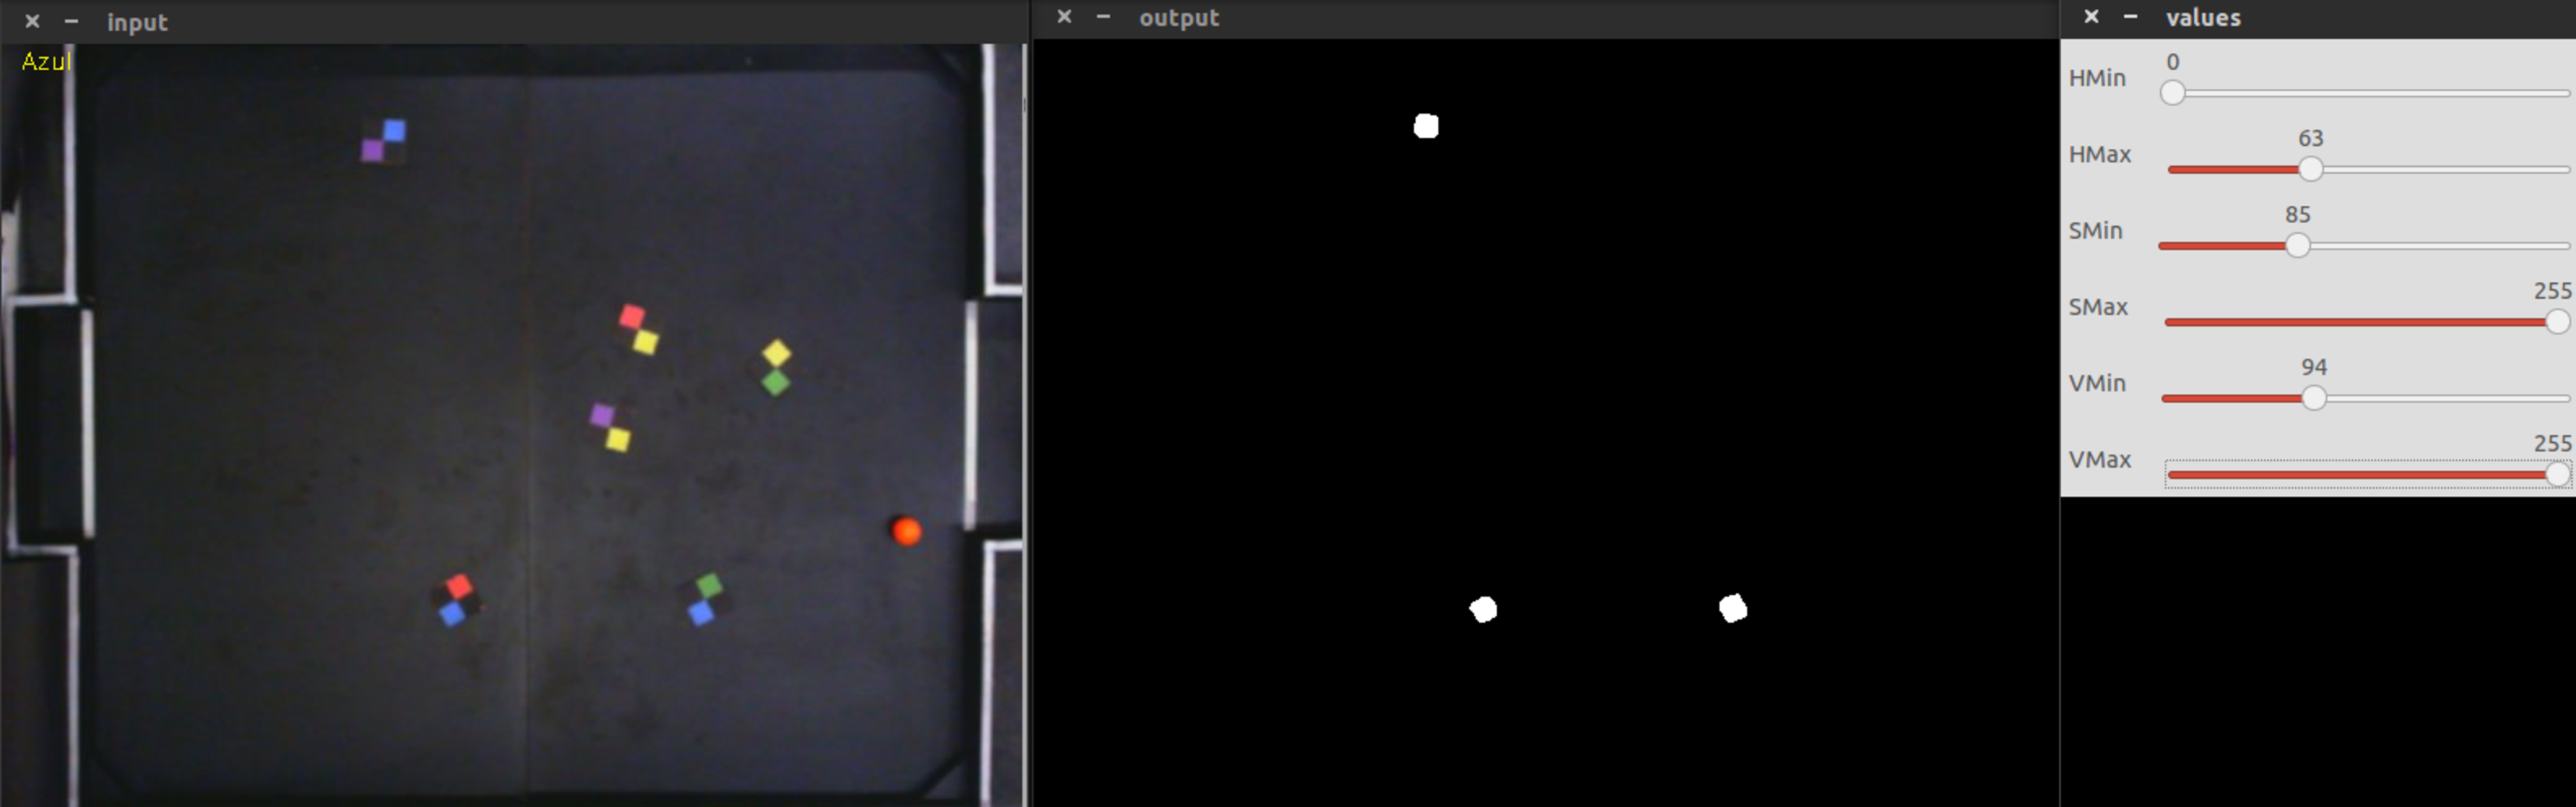
\includegraphics[width=0.8\textwidth]{calibration.pdf} 	
	\caption{Sistema de calibracao desenvolvido peloSIRLab \cite{VSSVision}}
	\label{SIRLabCalibracaoHSV}
\end{figure}

O atual sistema de visão computacional do SIRLab passou por algumas mudanças desde 2015 e conta com uma inteface e metodo de calibração diferentes\cite{VSSVision}. 
Como disponivel no repositorio online do Laboratorio, o atual sistema de calibração de cores utiliza o espaço de cores HSV, no lugar do RGB\cite{Rosa:2015}. A antiga inteface do sistema, feita inicialmente em ImGui deu lugar à nova, desenvolvida em Qt, como mostrado na Figura \ref{SIRLabNova}.
\begin{figure}[!h]
	\centering
	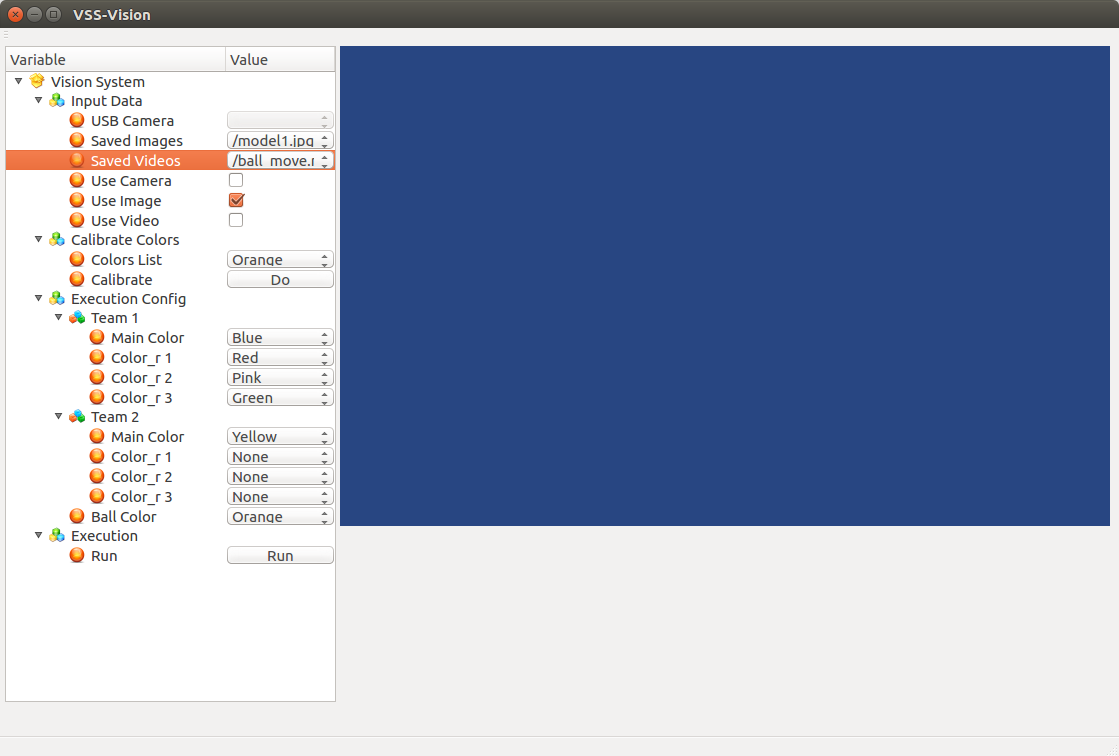
\includegraphics[width=0.5\textwidth]{vsssnovonormal.png} 	
	\caption{Nova interface do time da SIRLab \cite{VSSVision}}
	\label{SIRLabNova}
\end{figure}

O metodo de calibração de cores tambem foi modificado, segundo a equipe\cite{VSSVision} o sistema possibilita a calibragem de 8 cores, Laranja, Amarelo, Azul, Vermelho, Verde, Rosa, Roxo, Marrom. Após o usuário escolher uma cor para calibrar o mesmo deve encontrar um intervalo de cor, no espaço de cores HSV, que represente-a. Ao clicar na tela com o botão direito o sistema da um zoom na área para ajuste fino. A figura \ref{SIRLabNovaCalibracao} demonstra o novo metodo de calibração.

\begin{figure}[!h]
	\centering
	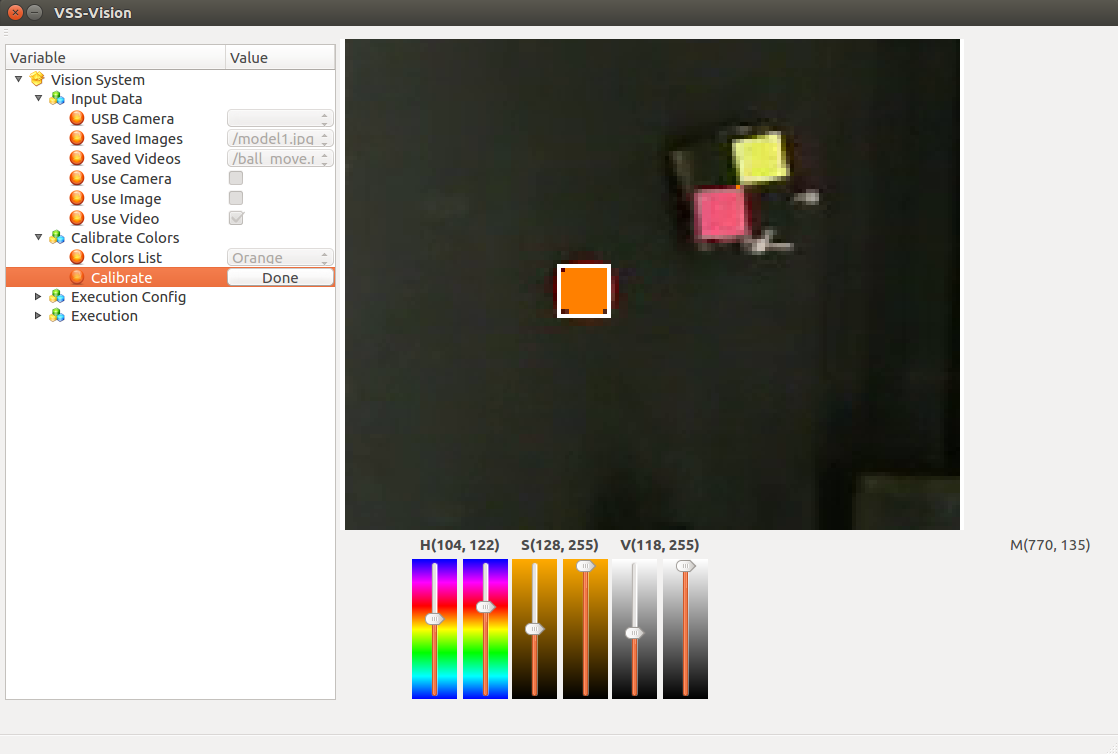
\includegraphics[width=0.5\textwidth]{vsssnovo.png} 	
	\caption{Calibração atual do time da SIRLab \cite{VSSVision}}
	\label{SIRLabNovaCalibracao}
\end{figure}


\section{Organização da Trabalho} \label{Sec:Organizacao}
No segundo capitulo encontra-se a fundamentação teorica do texto, contento sobre processamento de imagens referente à detecção de objetos e cores. A descrição da probabilidade usada no trabalho, na descoberta do tamanho desejavel dos objetos, além de uma breve descrição sobre o futebol de robôs e a descrição das tecnologias utilizadas no projeto.